\documentclass[12pt]{article}
\usepackage[english]{babel}
\usepackage[utf8x]{inputenc}
\usepackage{amsmath}
\usepackage{graphicx}
\usepackage[colorinlistoftodos]{todonotes}
\usepackage{hyperref}
\usepackage{color}
\hypersetup{
	colorlinks=true,
	linkcolor=blue,
	filecolor=magenta,      
	urlcolor=cyan,
}

\begin{document}
%---------------------------------------------------------------------------------------
%
%  Title
%
%---------------------------------------------------------------------------------------
\begin{titlepage}
	
	\centering
	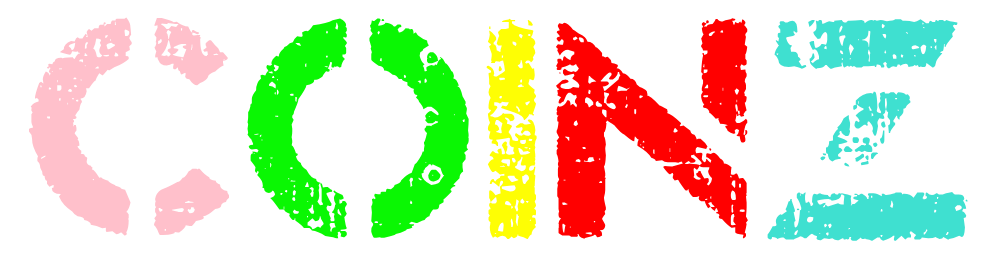
\includegraphics[scale=0.3]{coinz.png}\\[2cm]
	
	\textsc{\large School of Informatics, University of Edinburgh}\\[0.3cm]
	
	\hrule height 0.05cm
	\vspace{1cm}
	{\huge \bfseries Informatics Large Practical Coursework 2}
	\vspace{1cm}
	\hrule height 0.05cm
	
	\vspace{2cm}
	{\Large \textbf{CHENG LI}}\\[0.5cm]
	{\Large \textbf{s1603732}}\\[2cm]
	
	{\Large \today}\\[2cm]
		
\end{titlepage}
%---------------------------------------------------------------------------------------
%
%  Introduction
%
%---------------------------------------------------------------------------------------
\section{Introduction}
\paragraph{} This report describes the implementation of my Coinz game.
%---------------------------------------------------------------------------------------
%
%  Structure
%
%---------------------------------------------------------------------------------------
\section{Implementation Structure}

\subsection{Project Structure}
\subsubsection{Versions}
\hspace{12pt}\textbf{Android Studio: 3.1.4} \\
\null\hspace{12pt}\textbf{Gradle: 3.1.4} \\
\null\hspace{12pt}\textbf{Kotlin: 1.2.50} \\
\null\hspace{12pt}\textbf{Android SDK Tools: 26.1.1} \\
\null\hspace{12pt}\textbf{Android Platform Version: API 28 revision 6} \\
\null\hspace{12pt}\textbf{Firebase Core: 16.0.4}
\subsubsection{Emulator}
\hspace{12pt}\textbf{Emulator: Nexus 5X} \\
\null\hspace{12pt}\textbf{API: 26} \\
\null\hspace{12pt}\textbf{Target: Android 8.0 (Google Play)} \\
\null\hspace{12pt}\textbf{Screen size: 5.2} \\
\null\hspace{12pt}\textbf{Resolution: 1080 $\times$ 1920 (420 dpi)}
\subsubsection{App Structure}
\paragraph{$\bullet$}
See figure~\ref{fig:structure} on page~\pageref{fig:structure} for a general structure.
Blues rectangles represent essential activities, while the pink ones represent bonus activities. The yellow rectangle is the navigation drawer, which is not an activity, but plays a significant role in connecting activities.
\paragraph{$\bullet$}
More details are given at section~\ref{sec:activity} on page~\pageref{sec:activity}.
%---------------------------------------------------------------------------------------
%  Figure
\begin{figure}
	\centering
	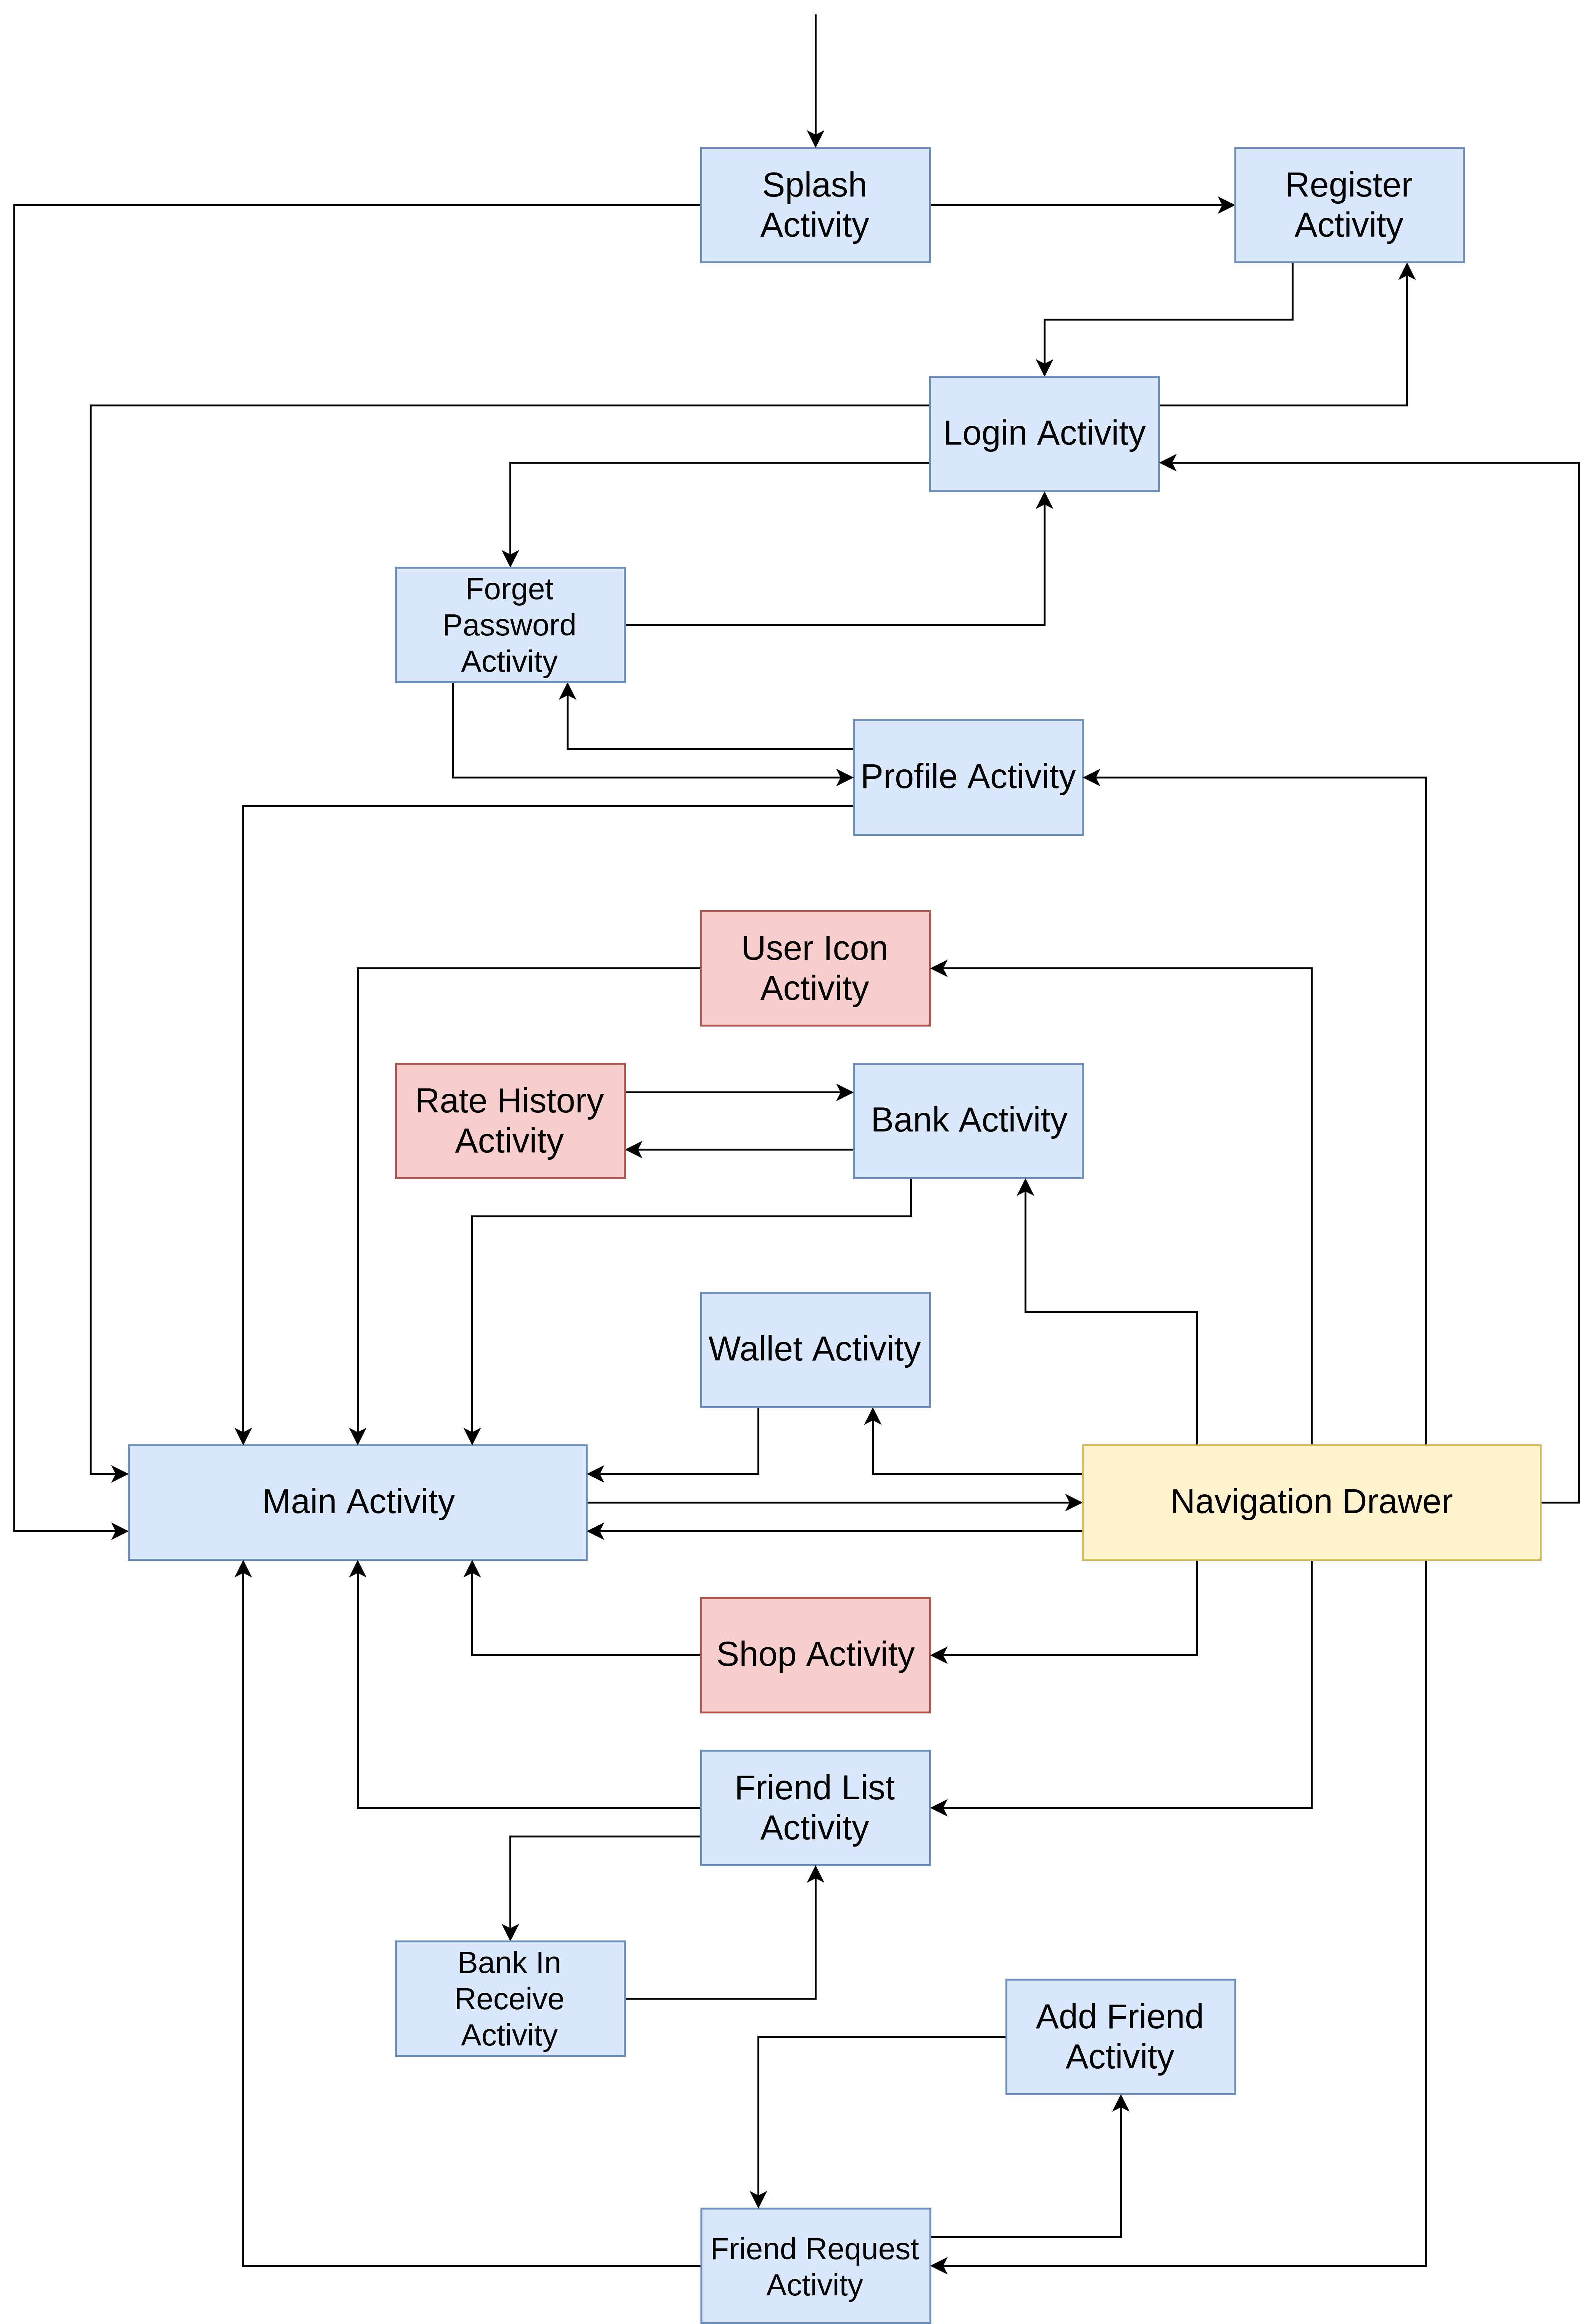
\includegraphics[scale=0.085]{Structure.png}
	\caption{\label{fig:structure}This is the structure of the app.}
\end{figure}
%  Figure
%---------------------------------------------------------------------------------------

\subsection{Database}
\subsubsection{Versions}
\hspace{12pt}\textbf{Firebase Firestore: 17.1.2} \\
\null\hspace{12pt}\textbf{Firebase Storage: 16.0.4}
\subsubsection{Structure}
\paragraph{}
See figure~\ref{fig:data} on page~\pageref{fig:data} for a general structure. \\ \\
\null\hspace{12pt}$\bullet$\enskip\textbf{Firebase Firestore:} See figure~\ref{fig:database} on page~\pageref{fig:database} for an example. Stores all data except user icon images. Yellow folders represent the collections; blue-white rectangles represents documents, where the blue bars show how each document is named and the white parts show what data together with the types are stored in each document. \\
\null\hspace{12pt}$\bullet$\enskip\textbf{Firebase Storage:} See figure~\ref{fig:storage} on page~\pageref{fig:storage} for an example. Stores only user icon images. Users would have icon image files named as their email addresses stored in the yellow folder, if they upload their icon images.
%---------------------------------------------------------------------------------------
%  Figure
\begin{figure}
	\centering
	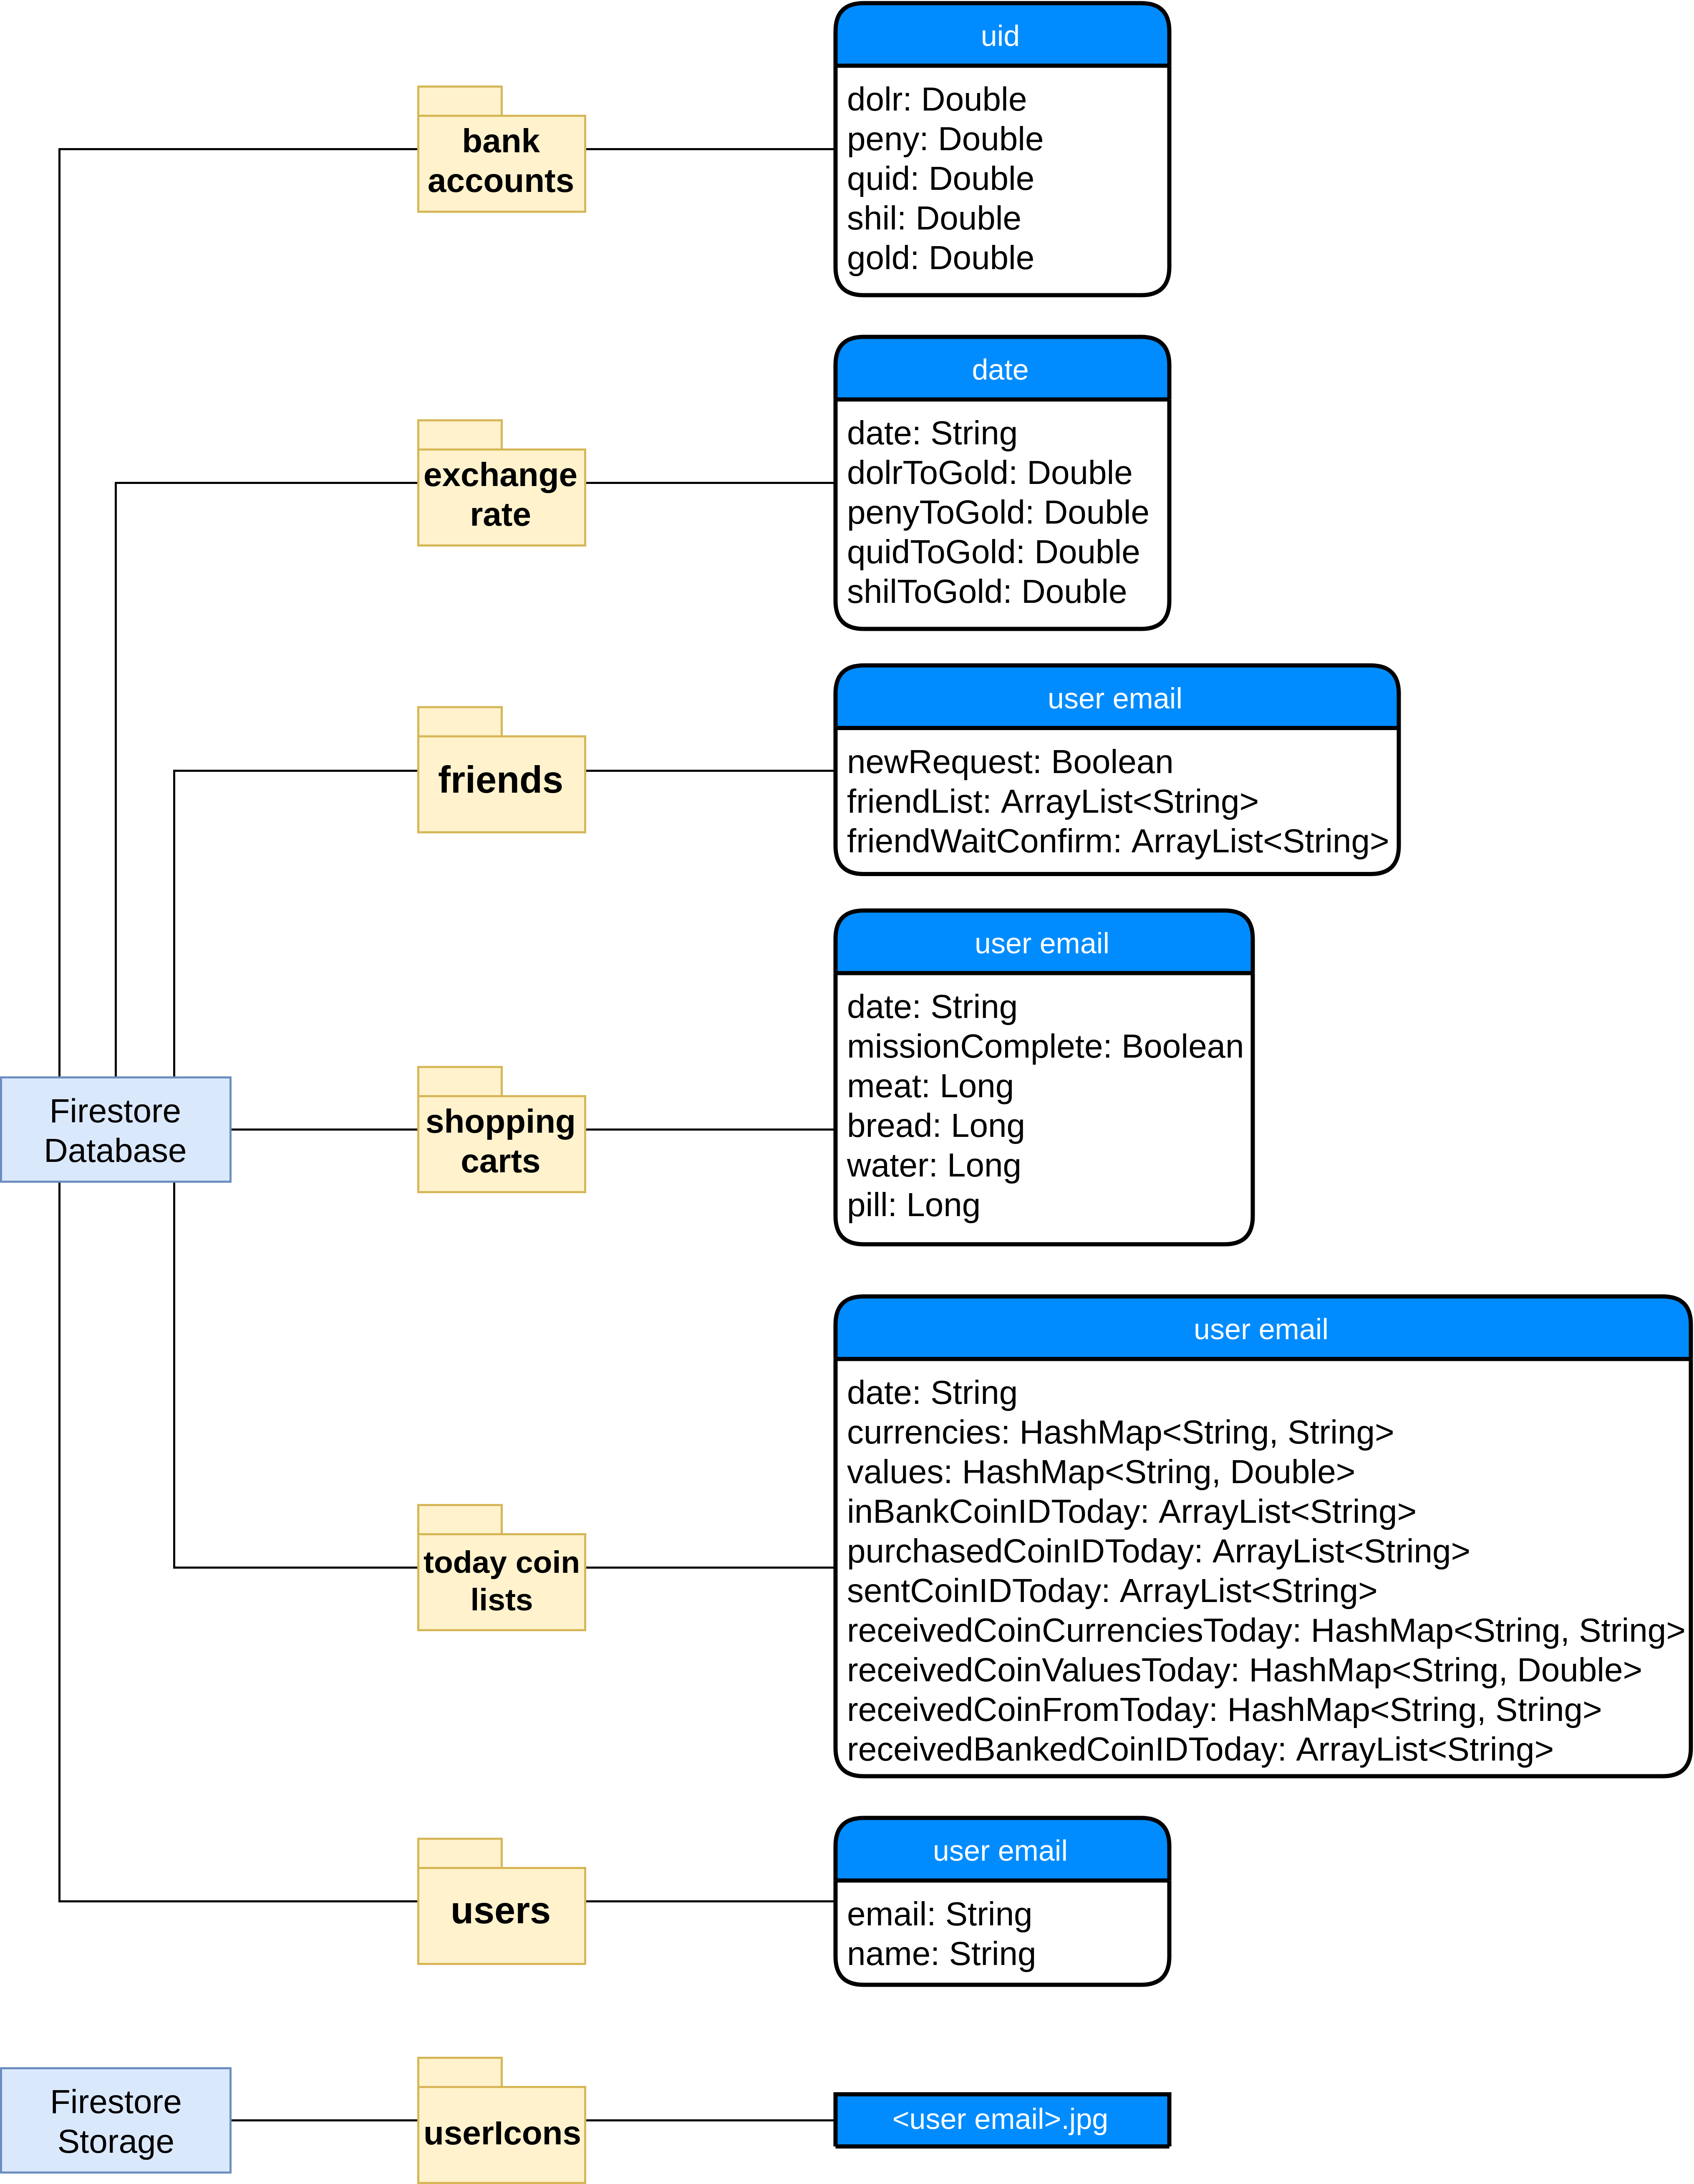
\includegraphics[scale=0.1]{Data.png}
	\caption{\label{fig:data}This is the structure of the database.}
\end{figure}
\begin{figure}
	\centering
	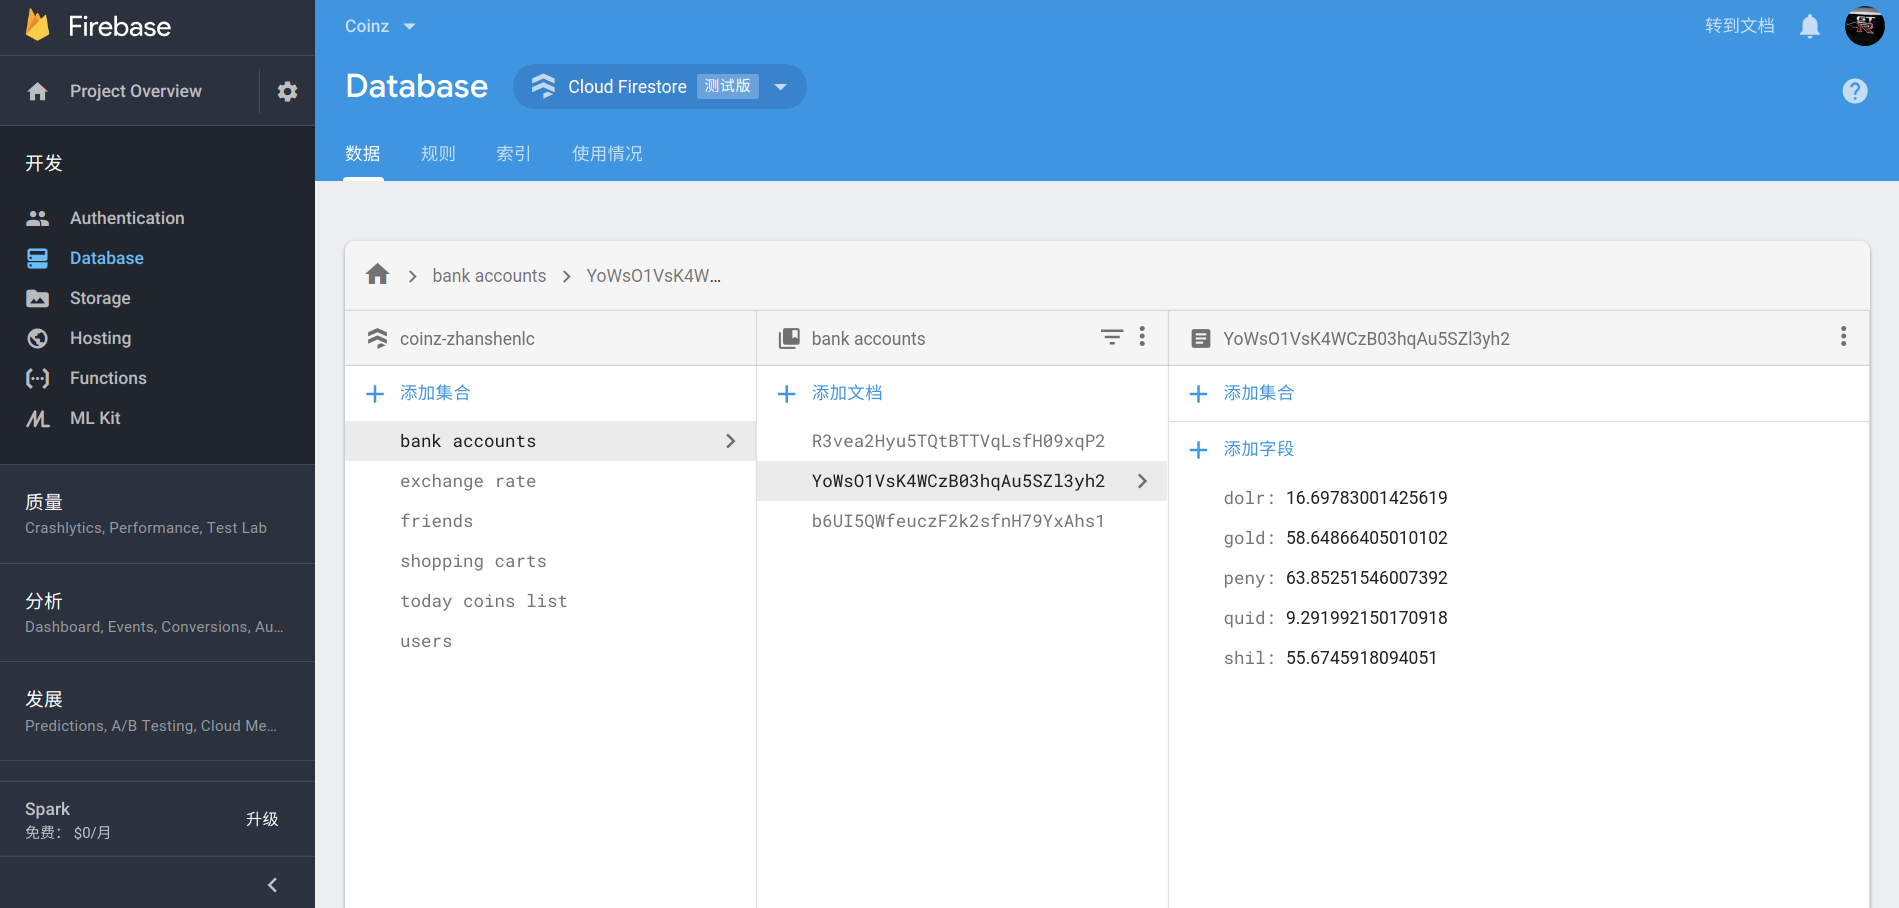
\includegraphics[scale=0.2]{Database.png}
	\caption{\label{fig:database}This is an example of a document in the Firebase Firestore.}
\end{figure}
\begin{figure}
	\centering
	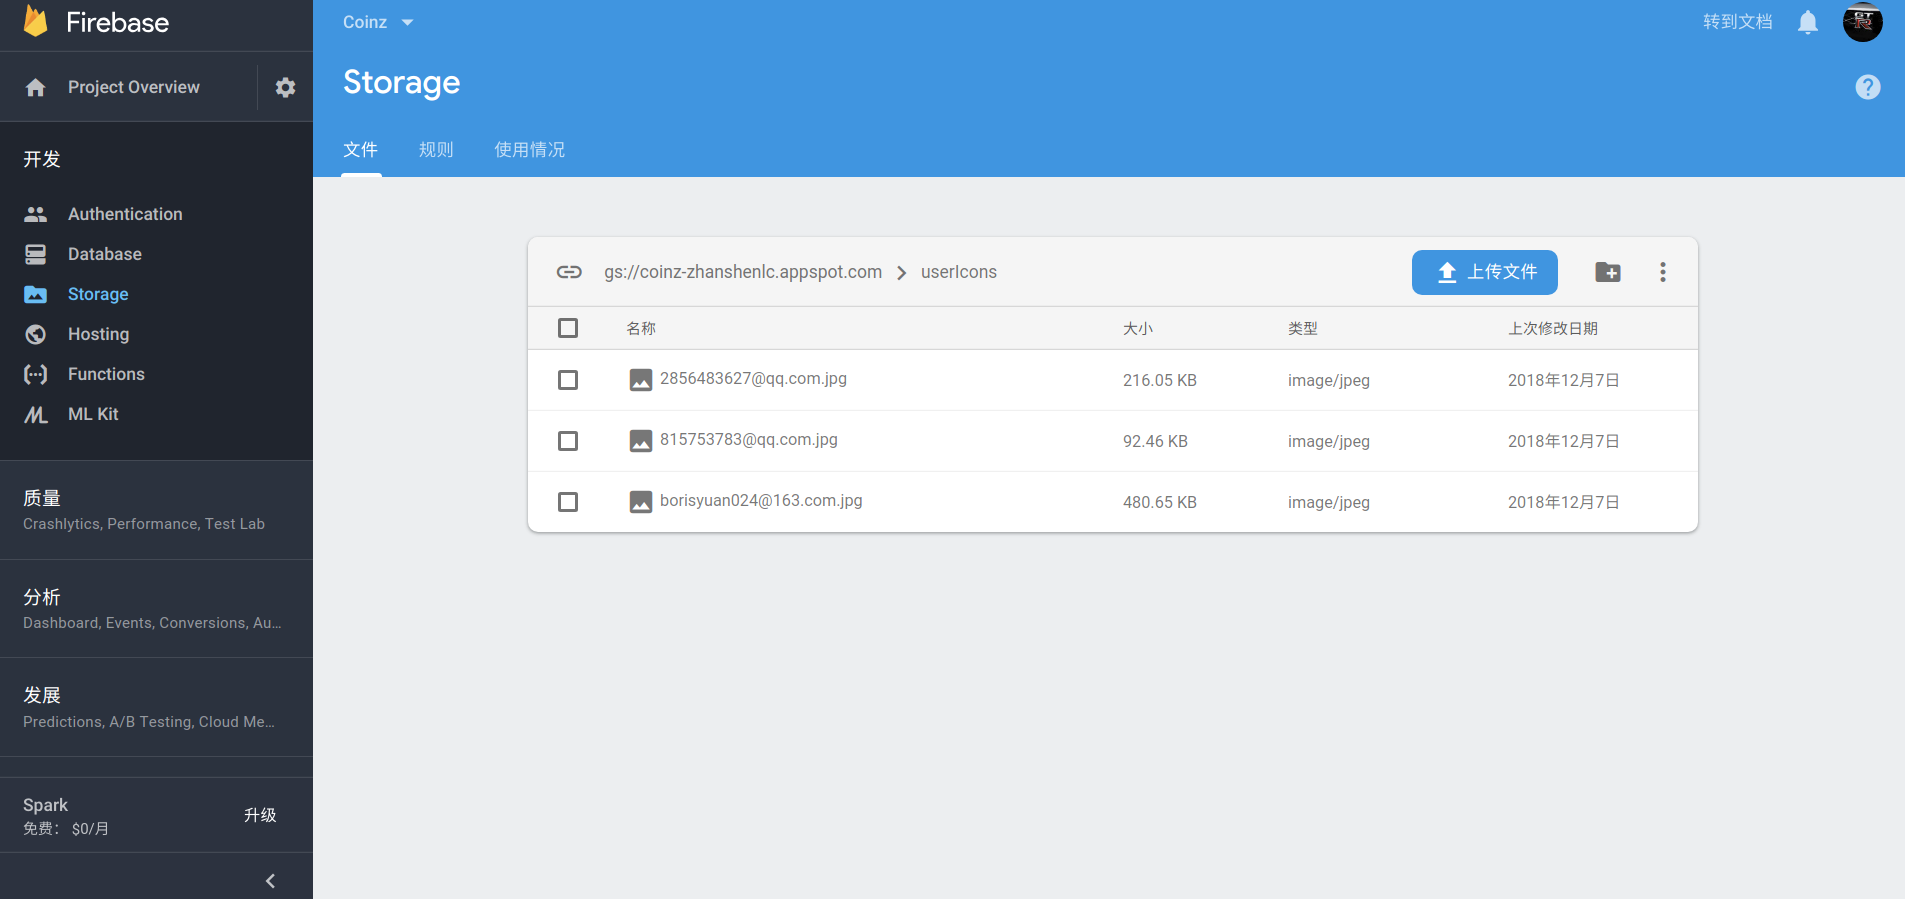
\includegraphics[scale=0.2]{Storage.png}
	\caption{\label{fig:storage}This is the userIcons folder in the Firebase Storage.}
\end{figure}
%  Figure
%---------------------------------------------------------------------------------------
\subsubsection{Firebase Firestore}
\paragraph{bank accounts:}
Since bank accounts do not involve other players, in order to improve level of security, it is set as the only collection where documents are named by user IDs generated by Firebase Authentication. Each document records user's balances for the four currencies and gold.
\paragraph{exchange rate:}
Since exchange rate is public, in order to access and retrieve the data more conveniently, it is set as the only collection where documents are named by dates. Each document records the date, and the corresponding rates from the four currencies to gold.
\paragraph{friends:}
From now on, all documents are named by the user email. Each document records whether there is a new friend request for the user. Also, each document records a friend list and a waiting confirmation list.
\paragraph{shopping carts:}
Each document records the date, and whether the user has completed the mission today. Also, each document records the current amounts of meat, bread, water and pill obtained.
\paragraph{today coin lists:}
Each document records the date, a currencies map and a values map, which are used for storing information of the coins user has collected today. Also, each document records lists which record the using of coins: banked in, purchased for food or sent to friends.
\paragraph{users:}
Each document records the email addresses and the names of users.
\paragraph{Main Functions used:} \textit{addSnapshotListener(), get(), update(), set()}
\subsubsection{Firebase Storage}
\paragraph{userIcons:} This folder stores icon images of all users as .jpg file and all images are named by the user email.
\paragraph{Main Functions used:} \textit{getFile(), putBytes()}

\subsection{User Authentication}
\subsubsection{Version}
\hspace{12pt}\textbf{Firebase Authentication: 16.0.5}
\subsubsection{Functions}
\paragraph{}
See figure~\ref{fig:auth} on page~\pageref{fig:auth} for the authentication console. An account is required to use the app. Email/Password is the only sign-in method for this app, and emails need to be verified before signing in. Also, users could receive a reset password email when they forget their passwords.
%---------------------------------------------------------------------------------------
%  Figure
\begin{figure}
	\centering
	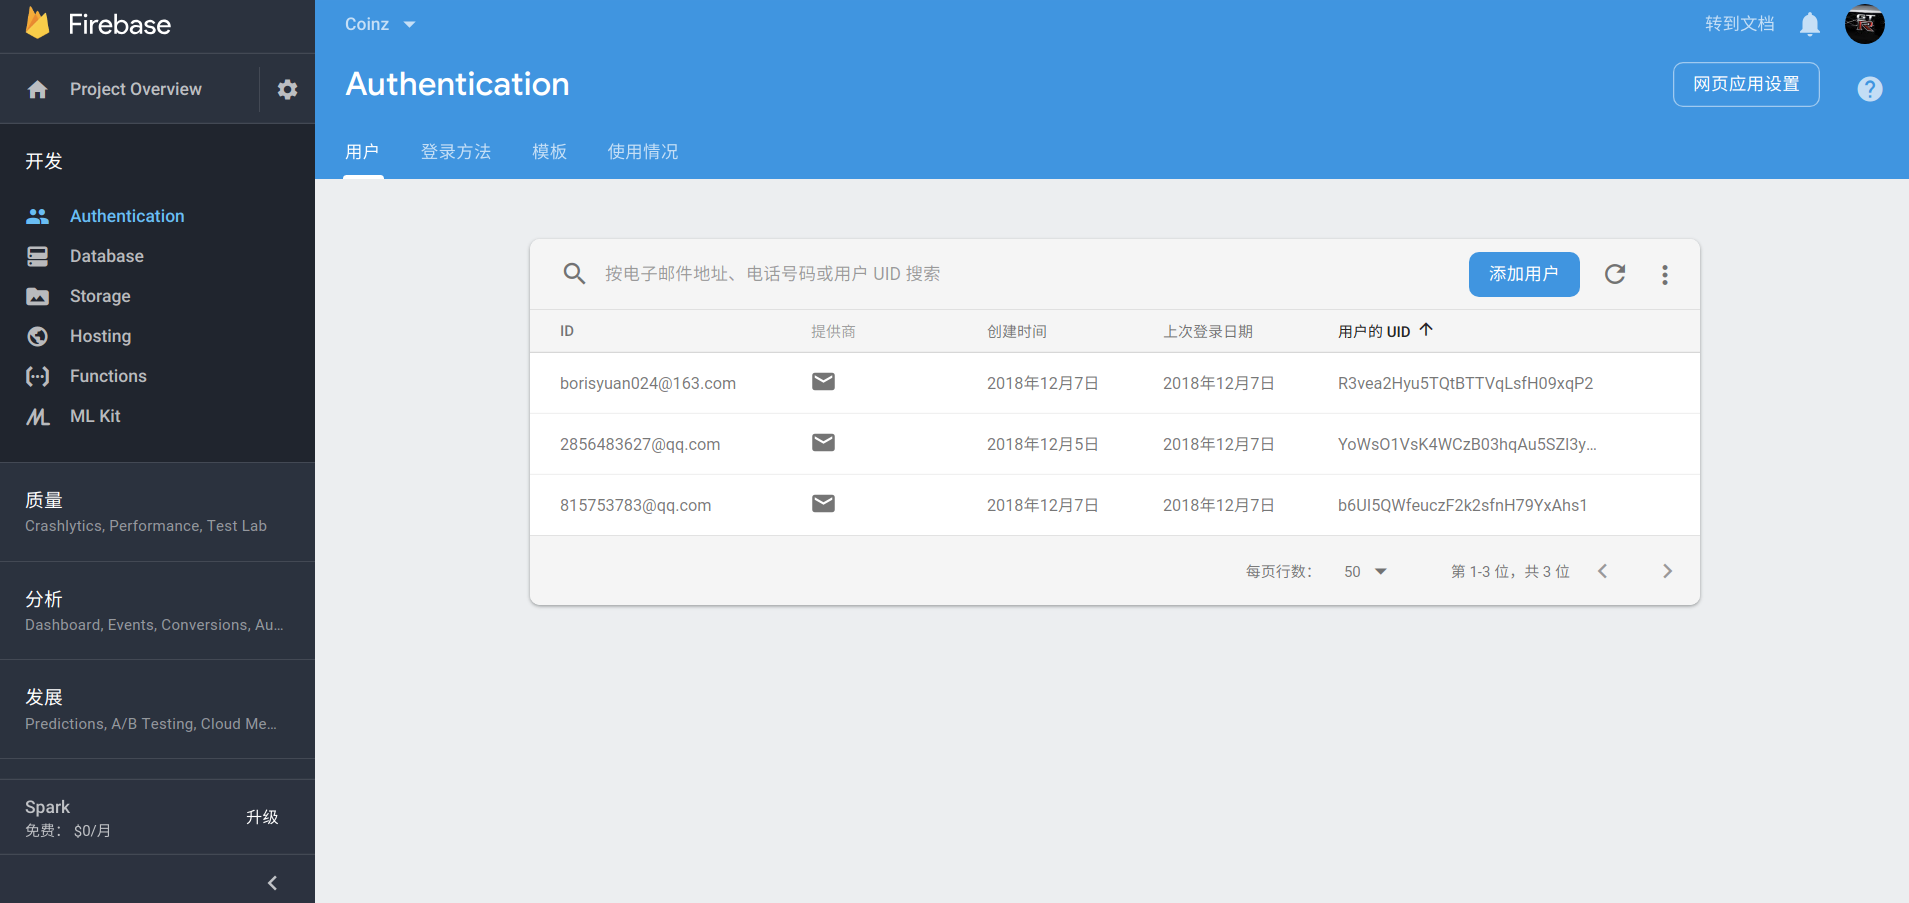
\includegraphics[scale=0.2]{Authentication.png}
	\caption{\label{fig:auth}This is the structure of the database.}
\end{figure}
%  Figure
%---------------------------------------------------------------------------------------

\subsection{Map}
\subsubsection{Versions}
\hspace{12pt}\textbf{Google Management System Play Location Service: 16.0.0} \\
\null\hspace{12pt}\textbf{Mapbox Android SDK: 6.6.1} \\
\null\hspace{12pt}\textbf{Mapbox Android Plugin Location Layer: 0.5.2}
\subsubsection{Map View}
\paragraph{}
Collecting coins on the map is the fundamental function of this game. A different set of 50 coins is scattered around George Square every day for players to collect. The map and location service are provided by Mapbox and Google, and coins are provided by \href{http://homepages.inf.ed.ac.uk/stg/coinz}{http://homepages.inf.ed.ac.uk/stg/coinz}.

%---------------------------------------------------------------------------------------
%
%  Activities
%
%---------------------------------------------------------------------------------------
\section{Activities}
\label{sec:activity}

\subsection{Splash Activity}
\subsubsection{General Functions}
\paragraph{}
See the first image of figure~\ref{fig:splash} on page~\pageref{fig:splash} for the Splash Activity. This activity displays a welcome screen for 4 seconds, and download the GeoJson file for the coins in background at the mean time. If there is a valid user logged in, the main activity is started; otherwise, the register activity is started.
%---------------------------------------------------------------------------------------
%  Figure
\begin{figure}
	\centering
	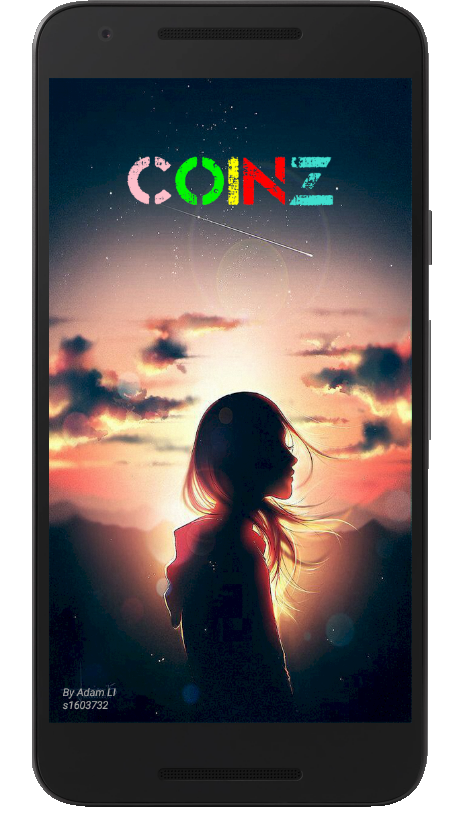
\includegraphics[scale=0.25]{SplashActivity.png}
	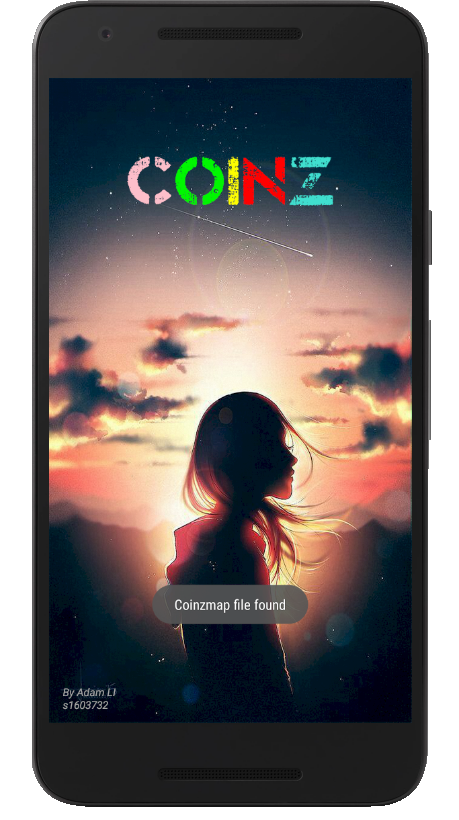
\includegraphics[scale=0.25]{SplashActivityFileFound.png}
	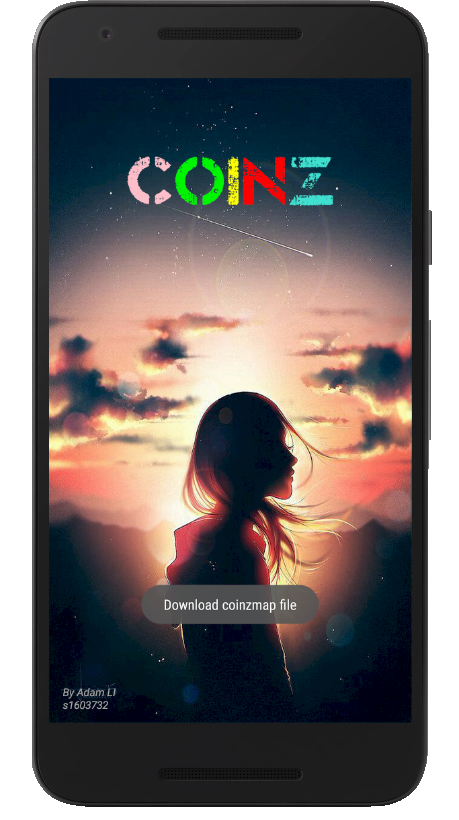
\includegraphics[scale=0.25]{SplashActivityNoFile.png}
	\caption{\label{fig:splash}Splash Activity}
\end{figure}
%  Figure
%---------------------------------------------------------------------------------------
\subsubsection{GeoJson File}
\paragraph{}
First, the app would check whether the last download date is the same as today's date and whether the file is broken or not (by checking the file size). If the last download date is today and the file is not broken, which means there is a valid file, the second image of figure~\ref{fig:splash} on page~\pageref{fig:splash} would be seen; otherwise, the app would download the newest file and update the last download date, and the third image of figure~\ref{fig:splash} on page~\pageref{fig:splash} would be seen.
\paragraph{}
The access and edit of the last download date was done by using \textit{getSharedPreference()}.
\paragraph{}
Downloading the coins file was done by implementing a \textit{AsyncTask} interface and a customised interface called \textit{DownloadCompleteListener}. Since we do not need to use the \textit{Progress} type and both of the \textit{Params} and the \textit{Result} types are String, i.e. \textit{AsyncTask$<$String, void, String$>$}, we only need to override \textit{doInBackground()} and \textit{onPostExecute()} functions. A URL string is passed in and data is parsed from the website as string, and when data is parsed, \textit{downloadComplete()} function overridden before hand is called \textit{DownloadCompleteListener} to store the data in a local file.
\paragraph{}
The check and update last download and download file methods are identical to the methods taught in the lectures. 

\subsection{Register Activity}
\paragraph{}
See the first image of figure~\ref{fig:registerLoginFp} on page~\pageref{fig:registerLoginFp} for Register Activity. You would be able to register an account if you input a valid email address (not registered by others and could receive verification email), a valid name (not empty) and a valid password (with 6 or more characters). After pressing the register button, users would receive a verification email and the app would start the login activity. Also, by clicking the text below, the app would directly start the login activity.
\paragraph{}
When registering the user using Firebase Authentication, user data would also be created at the same time, which include one document in each of the three folders: users, bank accounts and friends. Documents in other folders would be created later.
%---------------------------------------------------------------------------------------
%  Figure
\begin{figure}
	\centering
	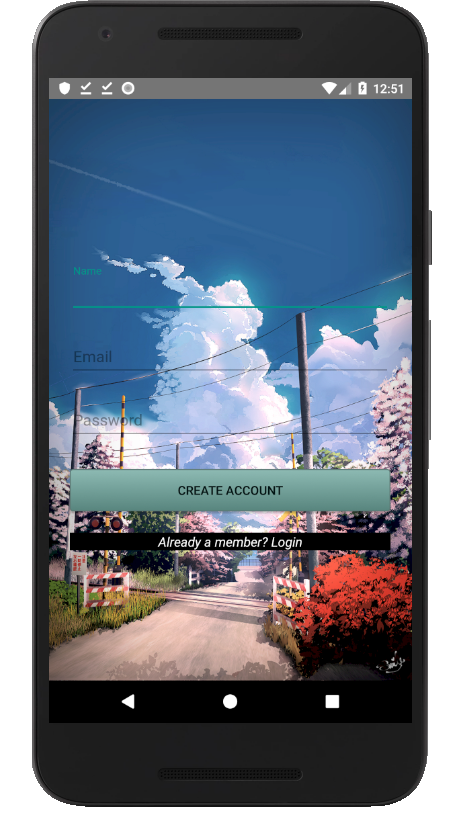
\includegraphics[scale=0.25]{RegisterActivity.png}
	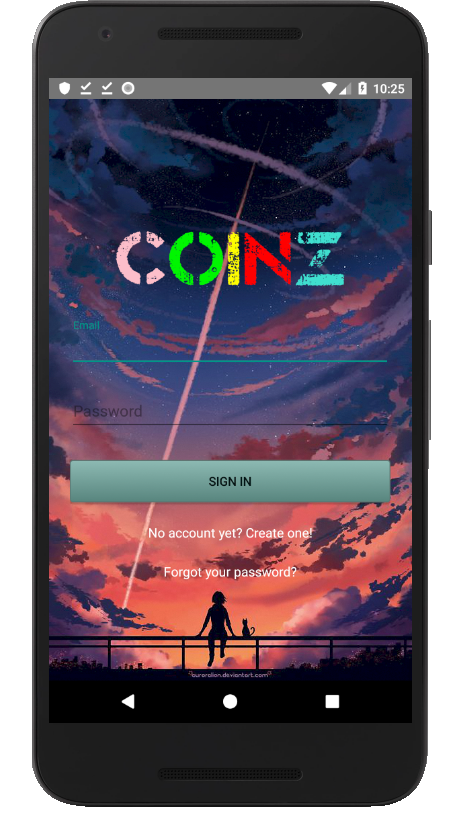
\includegraphics[scale=0.25]{LoginActivity.png}
	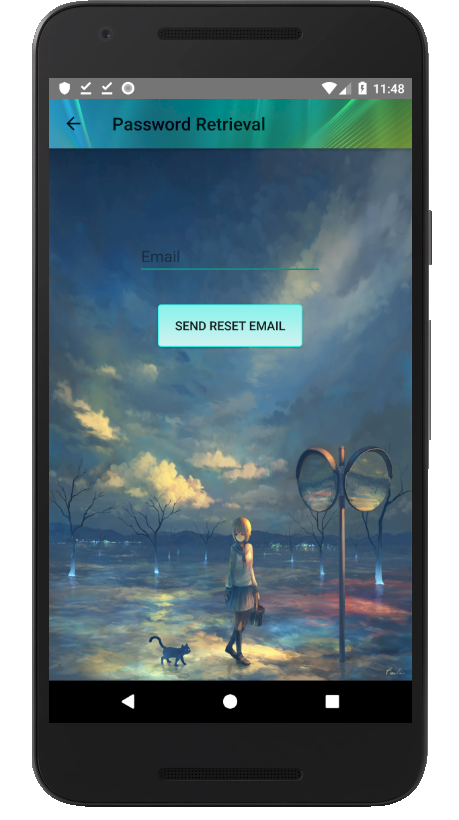
\includegraphics[scale=0.25]{ForgetPassword.png}
	\caption{\label{fig:registerLoginFp}Register Activity, Login Activity and Forget Password Activity}
\end{figure}
%  Figure
%---------------------------------------------------------------------------------------

\subsection{Login Activity}
\paragraph{}
See the second image of figure~\ref{fig:registerLoginFp} on page~\pageref{fig:registerLoginFp} for Login Activity. Users would not sign in unless the email they registered with is verified. Also, register activity and forget password activity (see the third image of figure~\ref{fig:registerLoginFp} on page~\pageref{fig:registerLoginFp}) could be reached at this point.

\subsection{Main Activity}
\subsubsection{General Functions}
\paragraph{}
The main activity is just a map with coins as markers on it (see the first image of figure~\ref{fig:main} on page~\pageref{fig:main}), together with a navigation drawer (see the second image of figure~\ref{fig:main} on page~\pageref{fig:main})
%---------------------------------------------------------------------------------------
%  Figure
\begin{figure}
	\centering
	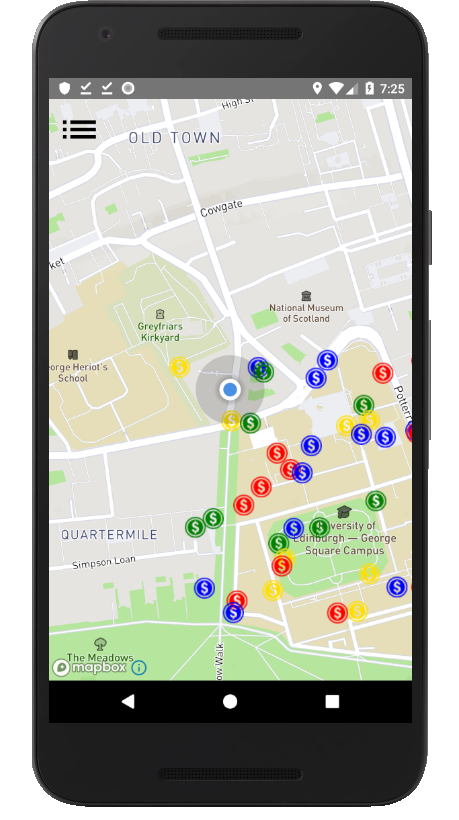
\includegraphics[scale=0.25]{MainActivity.png}
	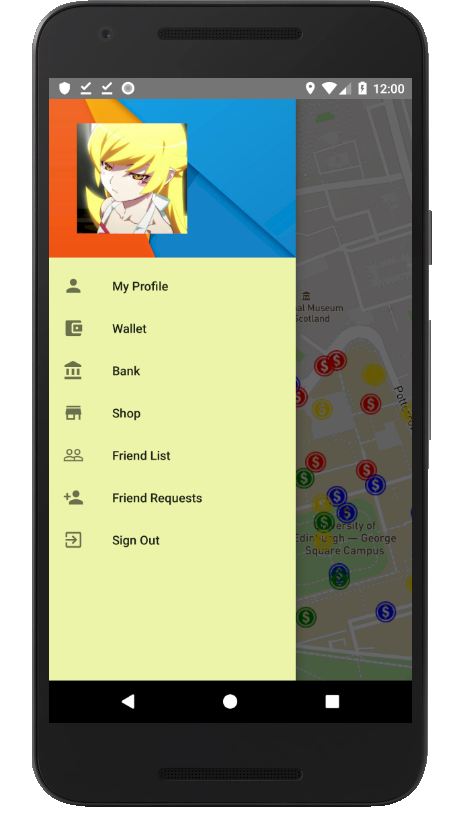
\includegraphics[scale=0.25]{NaviDrawer.png}
	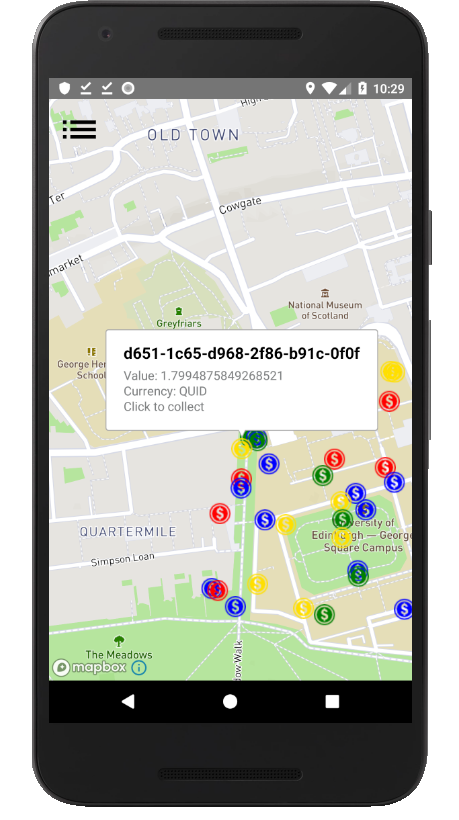
\includegraphics[scale=0.25]{CoinInfo.png}
	\caption{\label{fig:main}Main Activity}
\end{figure}
%  Figure
%---------------------------------------------------------------------------------------
\subsubsection{Map}
\paragraph{}
When the main activity is started, map view is initialised and the app would check whether the permission of location is granted or not and ask for permission if not. Then, the location service is initialised by \textit{initialiseLocationEngine()} and \textit{initialiseLocationLayer()} functions.
\paragraph{}
For the \textit{onMapReady()} function, the app would parse user's today coin lists data and check the date. If the date is not today or there is no available data in Firestore, a new \textit{CoinToday} class with date set as today would be uploaded to the cloud; otherwise, user's collected coins information would be parsed. Coins in today's GeoJson file would be shown on map in marker format if they have not been collected by the user. Each time a coin marker is clicked, an info window would pop up to show information of that coin (see the third image of figure~\ref{fig:main} on page~\pageref{fig:main}). User needs to click the info window in order to make a collection. If distance between user and coin is less than 25m, the coin would be successfully collected, the database would be updated (\textit{currencies} and \textit{values} HashMaps would both add one instance) with the collection and the collected coin marker would be removed by using the function \textit{remove()}.
\subsubsection{Distance by Longitude and Latitude}
\paragraph{Haversine Formula:}\mbox{}\\
\null\hspace{12pt} $a = sin^2(\frac{\Delta \phi}{2}) + cos\phi_1 \cdot cos\phi_2 \cdot sin^2(\frac{\Delta \lambda}{2})$ \\
\null\hspace{12pt} $c = 2 \cdot atan2(\sqrt{a}, \sqrt{1 - a})$ \\
\null\hspace{12pt} $d = R \cdot c$ \\
\null\hspace{12pt} where $\phi$ is latitude, $\lambda$ is longitude, R is earth's radius (mean radius = 6713 km); all angles need to be in radians
\subsubsection{Navigation Drawer}
\paragraph{}
Navigation Drawer could be opened either by clicking the top left image button or by dragging the screen from left edge to right. It is a hub of switches with access to all the other activities. Everything, including the user icon image is clickable.
\subsubsection{Daily Renewal}
\paragraph{}
The coins information updates daily, so users who are still playing the game at midnight would be notified to restart the game in order to obtain the latest version.

\subsection{\color{red}User Icon Activity}
\paragraph{}
It is a bonus feature not mentioned in the design, which allows users to customise their own user icons.
\paragraph{}
See figure~\ref{fig:userIcon} on page~\pageref{fig:userIcon}. Images which are not squares could be cropped as square and uploaded to Firebase Storage by the app.
%---------------------------------------------------------------------------------------
%  Figure
\begin{figure}
	\centering
	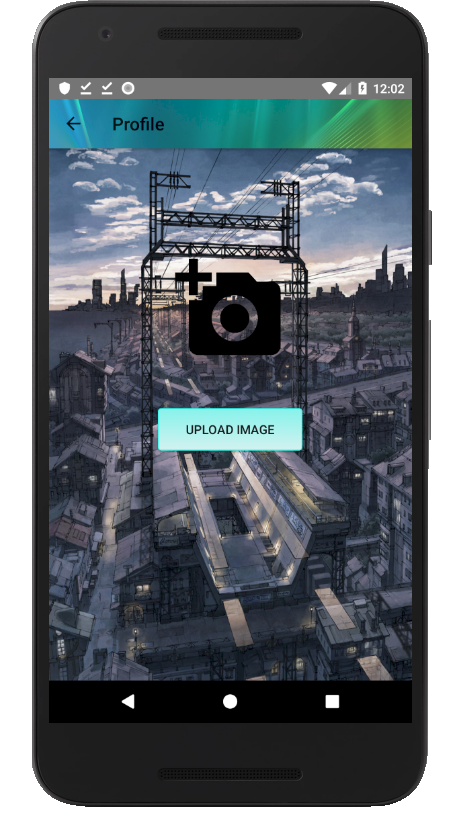
\includegraphics[scale=0.25]{UserIconActivity.png}
	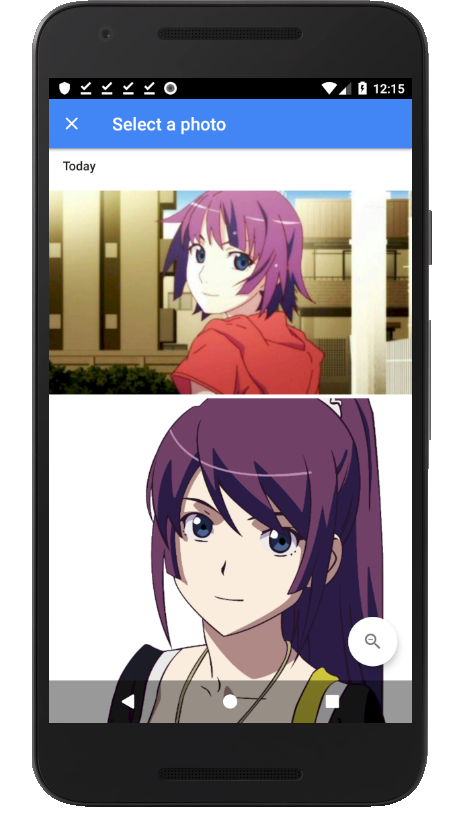
\includegraphics[scale=0.25]{Gallery.png}
	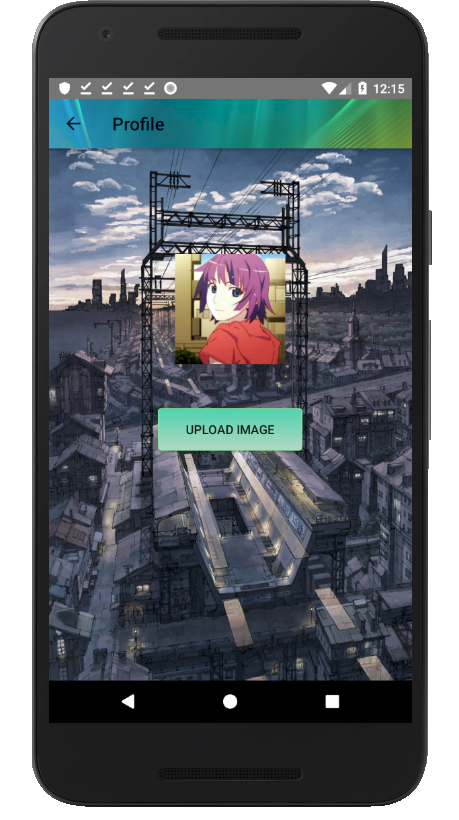
\includegraphics[scale=0.25]{UserIcon.png}
	\caption{\label{fig:userIcon}User Icon Activity}
\end{figure}
%  Figure
%---------------------------------------------------------------------------------------

\subsection{Profile Activity}
\paragraph{}
See the first image of figure~\ref{fig:profileWallet} on page~\pageref{fig:profileWallet}. It is a basic activity that allows users to view their emails and names and to make name and password changes.
%---------------------------------------------------------------------------------------
%  Figure
\begin{figure}
	\centering
	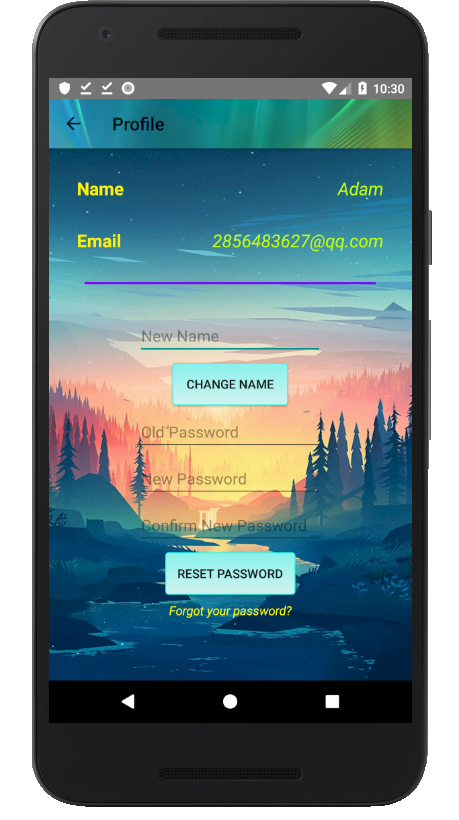
\includegraphics[scale=0.25]{Profile.png}
	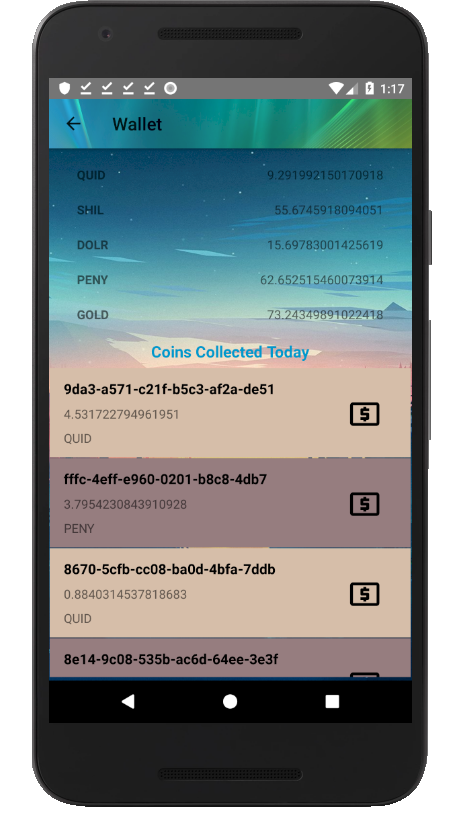
\includegraphics[scale=0.25]{Wallet.png}
	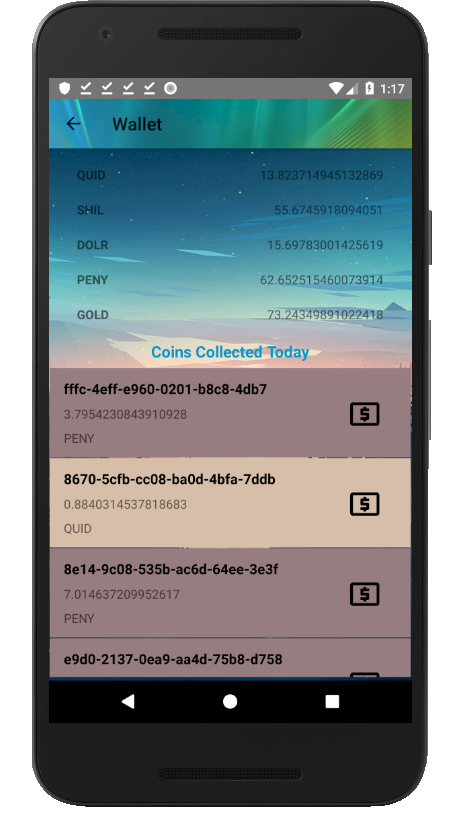
\includegraphics[scale=0.25]{WalletCollect.png}
	\caption{\label{fig:profileWallet}Profile Activity and Wallet Activity}
\end{figure}
%  Figure
%---------------------------------------------------------------------------------------

\subsection{Wallet Activity}
\paragraph{}
Wallet activity could not be started unless today's mission in shop activity is completed. It shows balance of users' bank accounts and coins (see the second image of figure~\ref{fig:profileWallet} on page~\pageref{fig:profileWallet}) that could be banked in (collected and did not used in buying things or sending to friends). Also, if a user banks in a coin, the coin would disappear from the coin list and the corresponding balance would increase (see the third image of figure~\ref{fig:profileWallet} on page~\pageref{fig:profileWallet}). Data are also updated to Firestore instantly.

\subsection{Bank Activity}
\subsubsection{General Functions}
\paragraph{}
Bank activity allows users to make currency exchanges, and check today and previous exchange rates.
\subsubsection{Exchange Rates}
\paragraph{}
Exchange rate is randomly (with reasonable fluctuations) generated automatically by the first user who starts the bank activity everyday (generate a set of rates and then upload to Firestore).
\subsubsection{Exchange}
\paragraph{}
All of the four currencies could be exchanged to gold and vice versa, and no direct exchange could be made among the four currencies. Also, bank would charge a fee of 5\% for each transaction. Transactions modes could be changed by clicking the buttons on the right of the exchange rates. See figure~\ref{fig:bank} on page~\pageref{fig:bank} for a transaction example, and please be aware of the colour changes.
%---------------------------------------------------------------------------------------
%  Figure
\begin{figure}
	\centering
	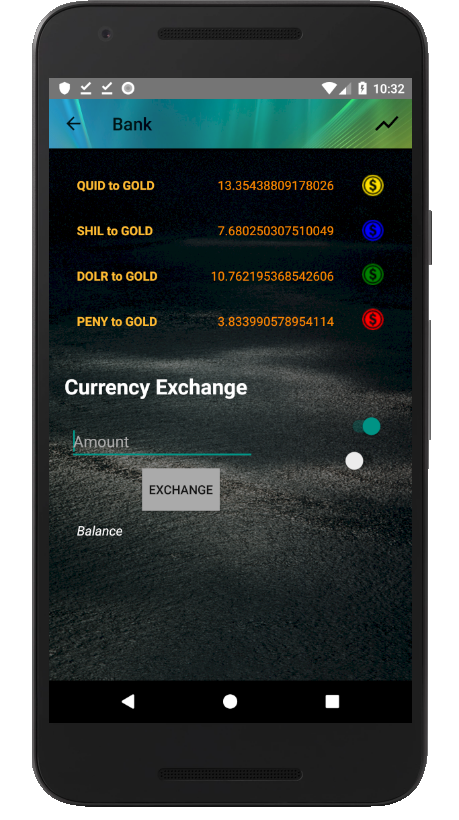
\includegraphics[scale=0.25]{BankActivity.png}
	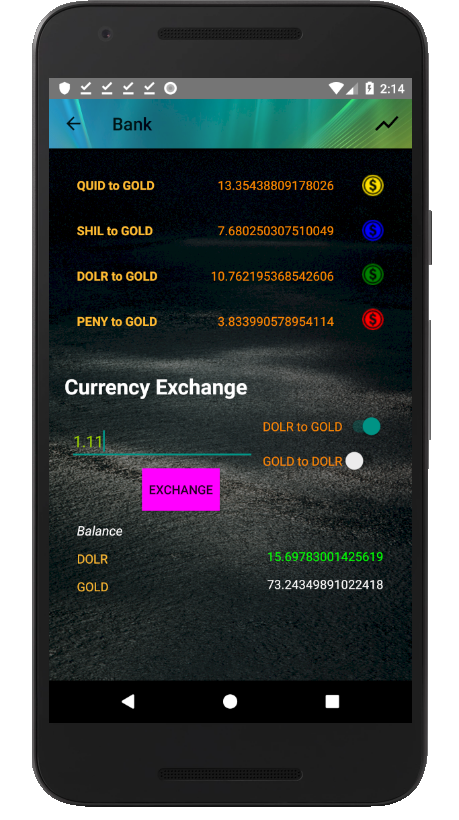
\includegraphics[scale=0.25]{BankActivityInputAmount.png}
	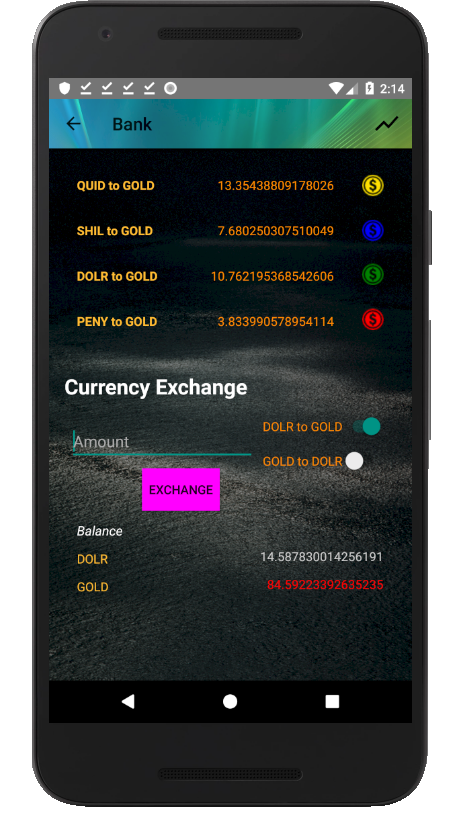
\includegraphics[scale=0.25]{BankActivityExchange.png}
	\caption{\label{fig:bank}Bank Activity}
\end{figure}
%  Figure
%---------------------------------------------------------------------------------------

\subsection{\color{red}Rate History Activity}
\paragraph{}
It is a bonus feature not mentioned in the design, which allows user to check previous exchange rates. See figure~\ref{fig:rateHistory} on page~\pageref{fig:rateHistory}.
%---------------------------------------------------------------------------------------
%  Figure
\begin{figure}
	\centering
	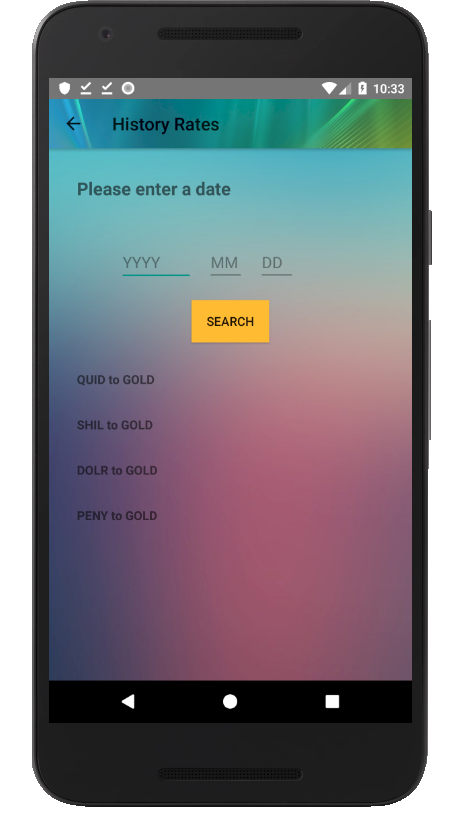
\includegraphics[scale=0.25]{HistoryRate.png}
	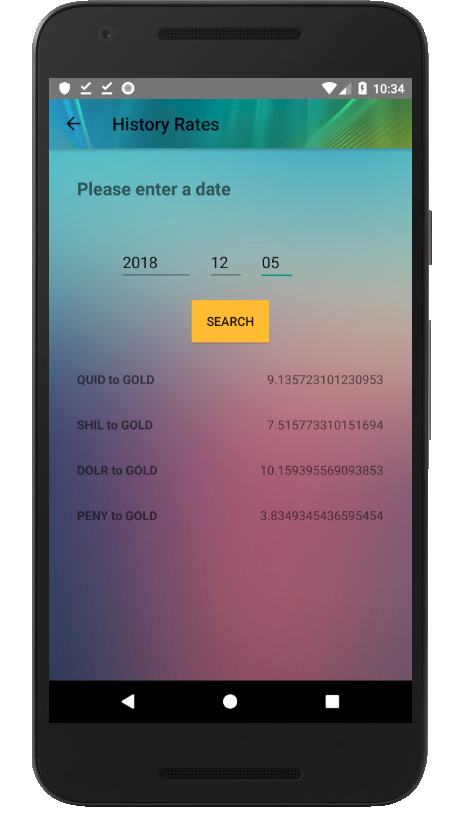
\includegraphics[scale=0.25]{HistoryRateSearch.png}
	\caption{\label{fig:rateHistory}Rate History Activity}
\end{figure}
%  Figure
%---------------------------------------------------------------------------------------

\subsection{\color{orange}Shop Activity}
\paragraph{}
It is a bonus feature mentioned in the design, which allows user to buy things with coins collected and complete daily mission. See figure~\ref{fig:shop} on page~\pageref{fig:shop} for a mission complete example.
\paragraph{}
A popup menu is used to store the coins which are available to pay with.
%---------------------------------------------------------------------------------------
%  Figure
\begin{figure}
	\centering
	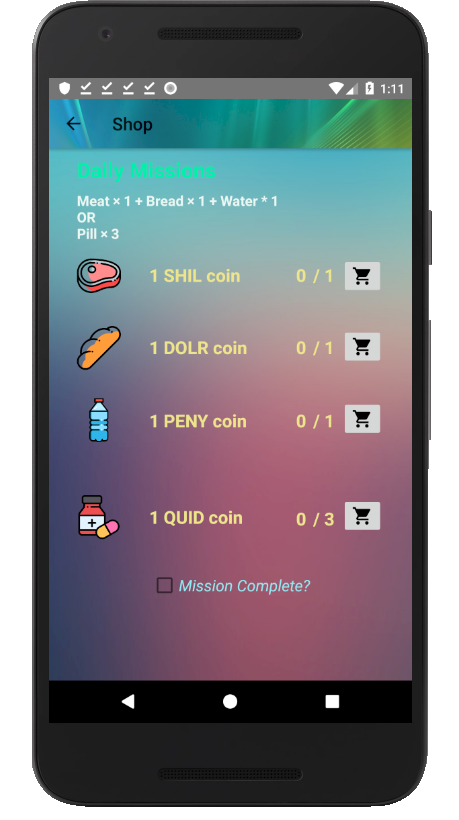
\includegraphics[scale=0.25]{shop.png}
	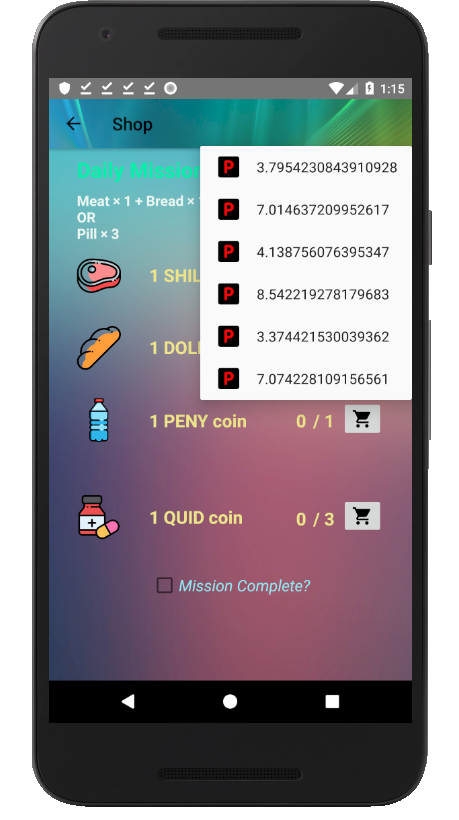
\includegraphics[scale=0.25]{shopBuy.png}
	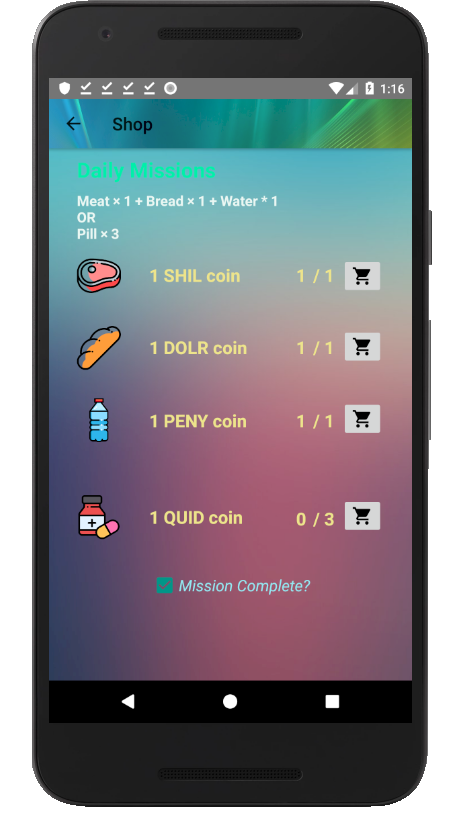
\includegraphics[scale=0.25]{missionComplete.png}
	\caption{\label{fig:shop}Shop Activity}
\end{figure}
%  Figure
%---------------------------------------------------------------------------------------

\subsection{Friend List Activity}
\paragraph{}
Friend List Activity shows all the friends user has added, and allow user to send coins to friends. See figure~\ref{fig:friend} on page~\pageref{fig:friend}.
\paragraph{}
A popup menu is used to store the coins which are available to send away.
%---------------------------------------------------------------------------------------
%  Figure
\begin{figure}
	\centering
	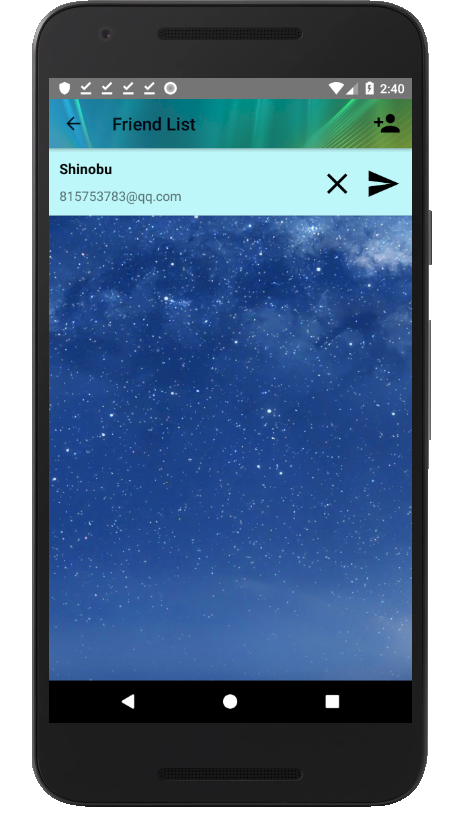
\includegraphics[scale=0.25]{Friend.png}
	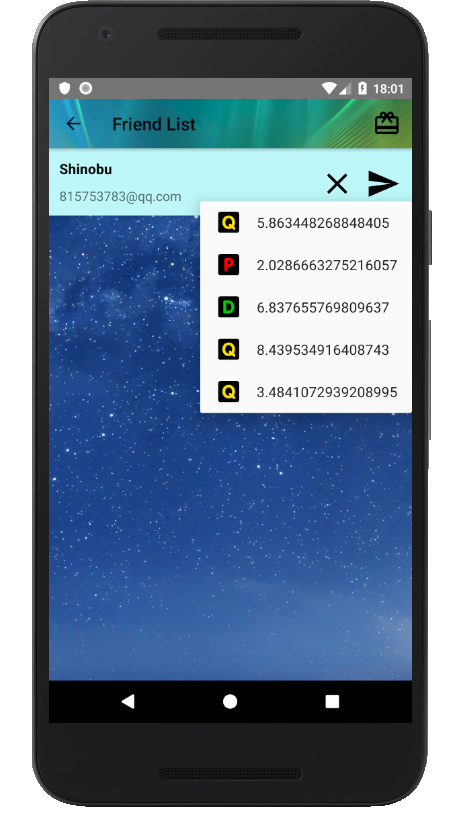
\includegraphics[scale=0.25]{FriendCoin.png}
	\caption{\label{fig:friend}Friend List Activity}
\end{figure}
%  Figure
%---------------------------------------------------------------------------------------

\subsection{Add Friend Activity}
\paragraph{}
Add friend activity allows users to add others as friend by sending a request. See the first image of figure~\ref{fig:requestAdd} on page~\pageref{fig:requestAdd}.
%---------------------------------------------------------------------------------------
%  Figure
\begin{figure}
	\centering
	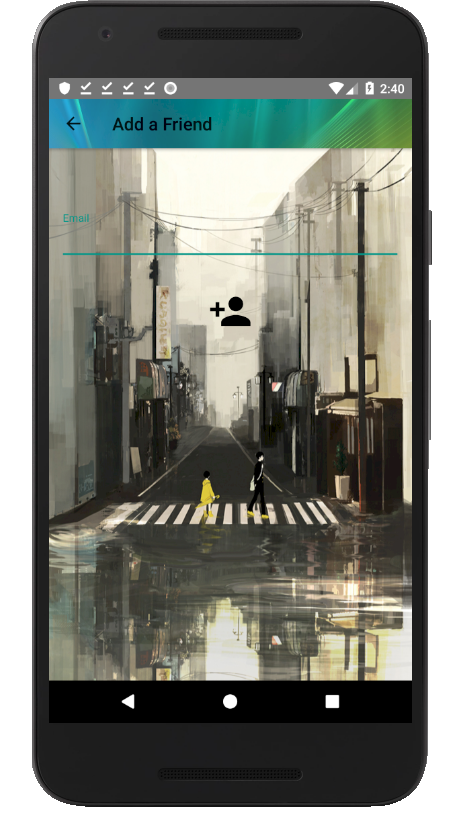
\includegraphics[scale=0.25]{AddFriend.png}
	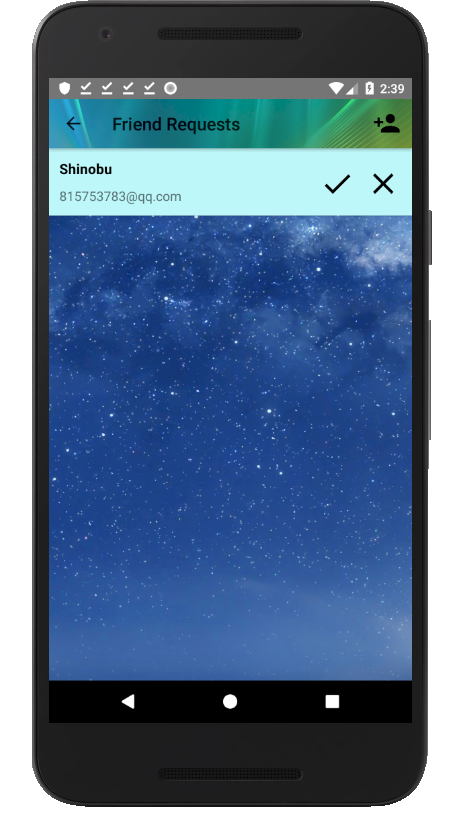
\includegraphics[scale=0.25]{FriendRequest.png}
	\caption{\label{fig:requestAdd}Add Friend Activity and Friend Request Activity}
\end{figure}
%  Figure
%---------------------------------------------------------------------------------------

\subsection{Friend Request List Activity}
\paragraph{}
Friend request list activity shows all the persons that are willing to add the user as a friend and provides the user options on whether to accept or refuse. See the second image of figure~\ref{fig:requestAdd} on page~\pageref{fig:requestAdd}.

\subsection{Unimplemented Bonus Features}
\paragraph{}
Due to limitation of time, those bonus features mentioned in the design was not realised: distance meter and pay-in helper.

%---------------------------------------------------------------------------------------
%
%  Acknowledgement
%
%---------------------------------------------------------------------------------------
\section{Acknowledgement}
\paragraph{Background Images:}
\href{www.pixiv.net}{www.pixiv.net}
\paragraph{Background Images:}
\href{https://www.pinterest.co.uk/}{https://www.pinterest.co.uk/}
\paragraph{Icon Images:} \href{https://www.flaticon.com/packs/simpleicon-ecommerce}{https://www.flaticon.com/packs/simpleicon-ecommerce}
\paragraph{Haversine Formula:}
\href{https://www.movable-type.co.uk/scripts/latlong.html}{https://www.movable-type.co.uk/scripts/latlong.html}
\paragraph{Popup Menu add images:}
\href{https://www.youtube.com/watch?v=ncHjCsoj0Ws}{https://www.youtube.com/watch?v=ncHjCsoj0Ws}
\paragraph{Mapbox:}
\href{https://www.youtube.com/watch?v=p9fOTyRqdV0\&t=652s}{https://www.youtube.com/watch?v=p9fOTyRqdV0\&t=652s} (whole series)
\paragraph{List View:}
\href{https://www.youtube.com/watch?v=EwwdQt3\_fFU\&t=823s}{https://www.youtube.com/watch?v=EwwdQt3\_fFU\&t=823s}
	
\end{document}
